% !TEX encoding = UTF-8 Unicode
% REMEMBER TO SET LANGUAGE!
\documentclass[a4paper,10pt,norsk]{article}
\usepackage[utf8]{inputenc}
\usepackage[norsk]{babel}

% Standard stuff
\usepackage{amsmath,graphicx,varioref,verbatim,amsfonts,geometry}
% colors in text
\usepackage[usenames,dvipsnames,svgnames,table]{xcolor}
% Hyper refs
\usepackage[colorlinks]{hyperref}

% Document formatting
\setlength{\parindent}{0mm}
\setlength{\parskip}{1.5mm}

%Color scheme for listings
\usepackage{textcomp}
\definecolor{listinggray}{gray}{0.9}
\definecolor{lbcolor}{rgb}{0.9,0.9,0.9}

%Listings configuration
\usepackage{listings}

%Hvis du bruker noe annet enn python, endre det her for å få riktig highlighting.
\lstset{
	backgroundcolor=\color{lbcolor},
	tabsize=4,
	rulecolor=,
	language=python,
        basicstyle=\scriptsize,
        upquote=true,
        aboveskip={1.5\baselineskip},
        columns=fixed,
	numbers=left,
        showstringspaces=false,
        extendedchars=true,
        breaklines=true,
        prebreak = \raisebox{0ex}[0ex][0ex]{\ensuremath{\hookleftarrow}},
        frame=single,
        showtabs=false,
        showspaces=false,
        showstringspaces=false,
        identifierstyle=\ttfamily,
        keywordstyle=\color[rgb]{0,0,1},
        commentstyle=\color[rgb]{0.133,0.545,0.133},
        stringstyle=\color[rgb]{0.627,0.126,0.941}
        }
        
\newcounter{subproject}
\renewcommand{\thesubproject}{\alph{subproject}}
\newenvironment{subproj}{
\begin{description}
\item[\refstepcounter{subproject}(\thesubproject)]
}{\end{description}}

%Lettering instead of numbering in different layers
%\renewcommand{\labelenumi}{\alph{enumi}}
\renewcommand{\thesubsection}{\alph{subsection}}

%opening
\title{MAT-INF1110 - Oblig 2}
\author{Joakim Flatby}

\begin{document}

\maketitle

%Oppg 1
\section{}

%Oppg 1a
\subsection{)}
\lstinputlisting{Task1a.py}

%Oppg 1b
\subsection{)}
\lstinputlisting{Task1b.py}

%Oppg 1c
\subsection{)}

(Kjører man denne koden vil man måtte krysse ut det første plottet for å se det andre, men jeg valgte likevel å gjøre det slik for å kunne inkludere plottene hver for seg i LaTeX, ettersom oppgaven ikke spesifiserte om de skulle ligge i samme plot eller ikke, og jeg synes dette så bedre ut.)

\lstinputlisting{Task1c.py}

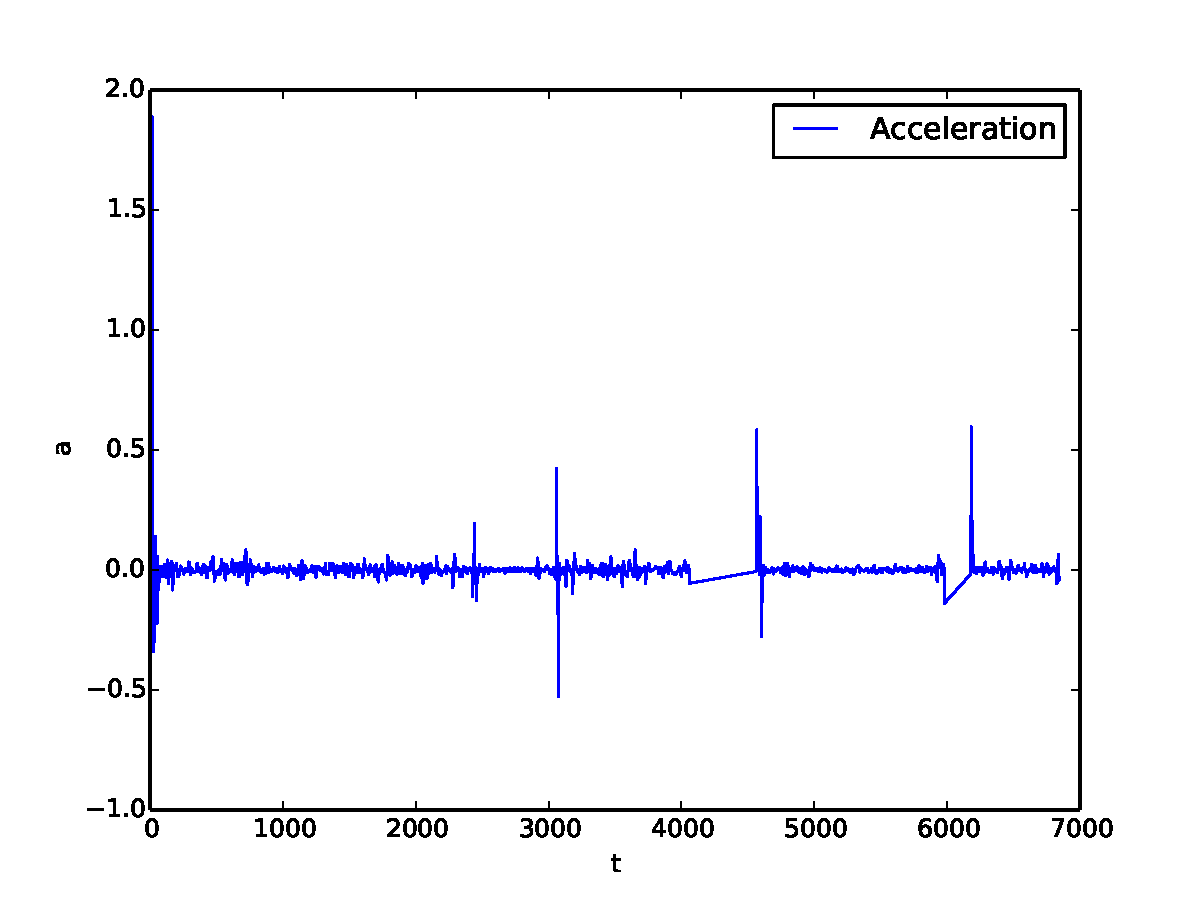
\includegraphics[scale=0.4]{a.pdf}
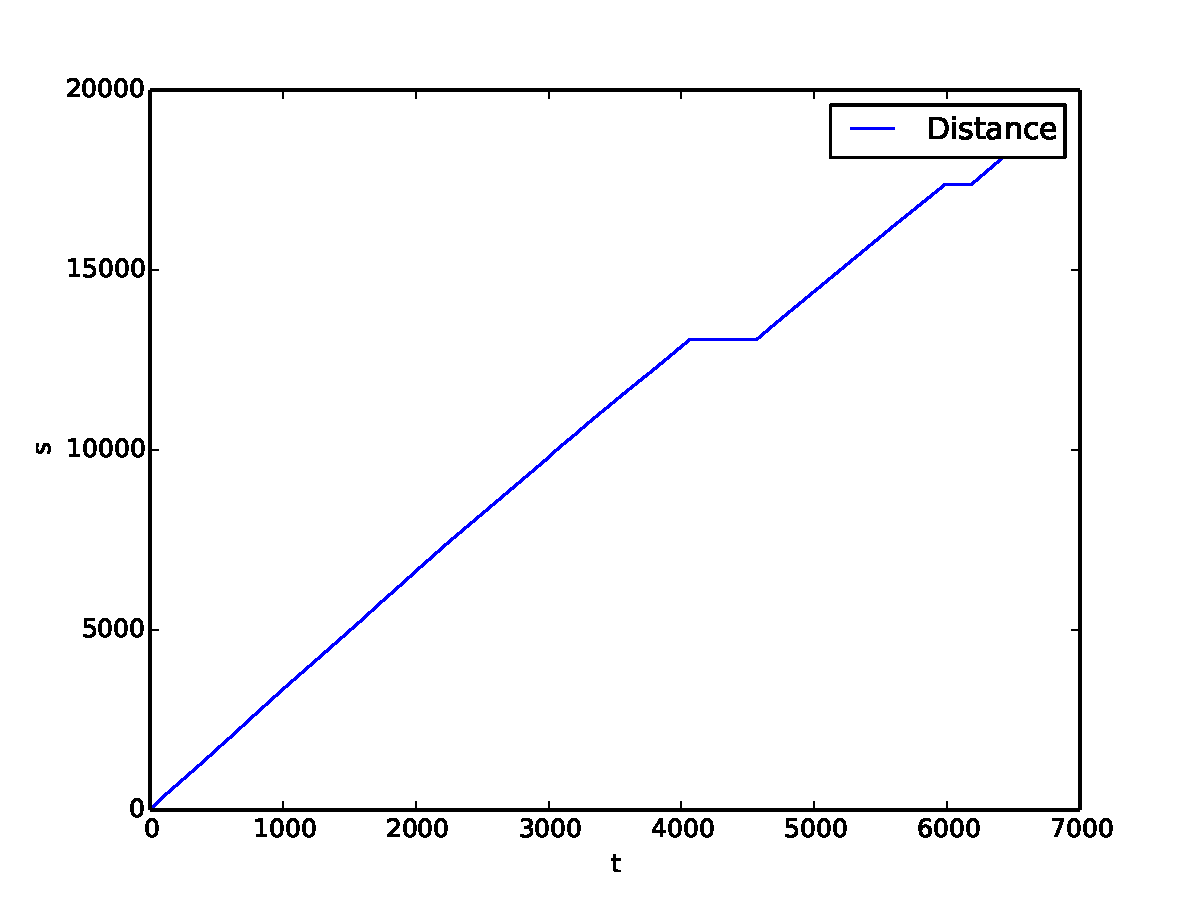
\includegraphics[scale=0.4]{s.pdf}

%Oppg 2
\section{}

%Oppg 2a
\subsection{)}
\[x' + x^{2} = 1\]
\[x'(t) + x(t)^{2} = 1\]
\[x'(t) = 1 - x(t)^{2}\]
\[\frac{x'(t)}{1 - x(t)^{2}} = 1\]
\[\int{\frac{x'(t)}{1 - x(t)^{2}} dt} = \int{1dt}\]
Substitusjon: \[u = x(t),\] \[du = x'(t)dt\]
\[\int{\frac{1}{1-u^{2}}du} = \int{\frac{1}{(1+u)(1-u)}du} = \int{\frac{a}{1+u}du} + \int{\frac{b}{1-u}du}\]

Dermed er også:
\[\frac{1}{(1+u)(1-u)} = \frac{a}{1+u} + \frac{b}{1-u}\]
\[1 = a(1-u) + b(1+u)\]
Setter inn $u=-1$ og $u=1$ 

og får at $a=\frac{1}{2}$ og $b=\frac{1}{2}$

\[\int{\frac{a}{1+u}du} + \int{\frac{b}{1-u}du} = \frac{1}{2}\int{\frac{1}{1+u}du} + \frac{1}{2}\int{\frac{1}{1-u}du} = t+C\]
\[\int{\frac{1}{1+u}du} + \int{\frac{1}{1-u}du} = 2t+2C\]
\[ln|1+u| - ln|1-u| = 2t + 2C\]
\[ln\left|\frac{1+u}{1-u}\right| = 2t+2C\]
\[\left|\frac{1+u}{1-u}\right| = e^{2(t+C)}\]
\[u = e^{2(t+C)} - ue^{2(t+C)} - 1\]
\[u + ue^{2(t+C)} = e^{2(t+C)} - 1\]
\[u(e^{2(t+C)} + 1) = e^{2(t+C)} - 1\]

\[x(t) = \frac{e^{2(t+C)} - 1}{e^{2(t+C)} + 1}\]
\[x(0) = \frac{e^{2(t+C)} - 1}{e^{2(t+C)} + 1} = 0\]
Dermed må C være lik 0:
\[x(0) = \frac{e^{0}-1}{e^{0} + 1} = \frac{1-1}{1+1} = \frac{0}{2} = 0\]
Og løsningen blir:
\[x(t) = \frac{e^{2t} - 1}{e^{2t} + 1}\]

%Oppg 2b
\subsection{)}
og
\subsection{)}
Her er den eksakte løsningen plottet sammen med de numeriske løsningene fra Eulers metode og Eulers midtpunktsmetode, programmert og plottet i Python.
Man ser utifra plottet at Eulers midtpunktsmetode gir en bedre tilnærming enn vanlig Eulers metode.

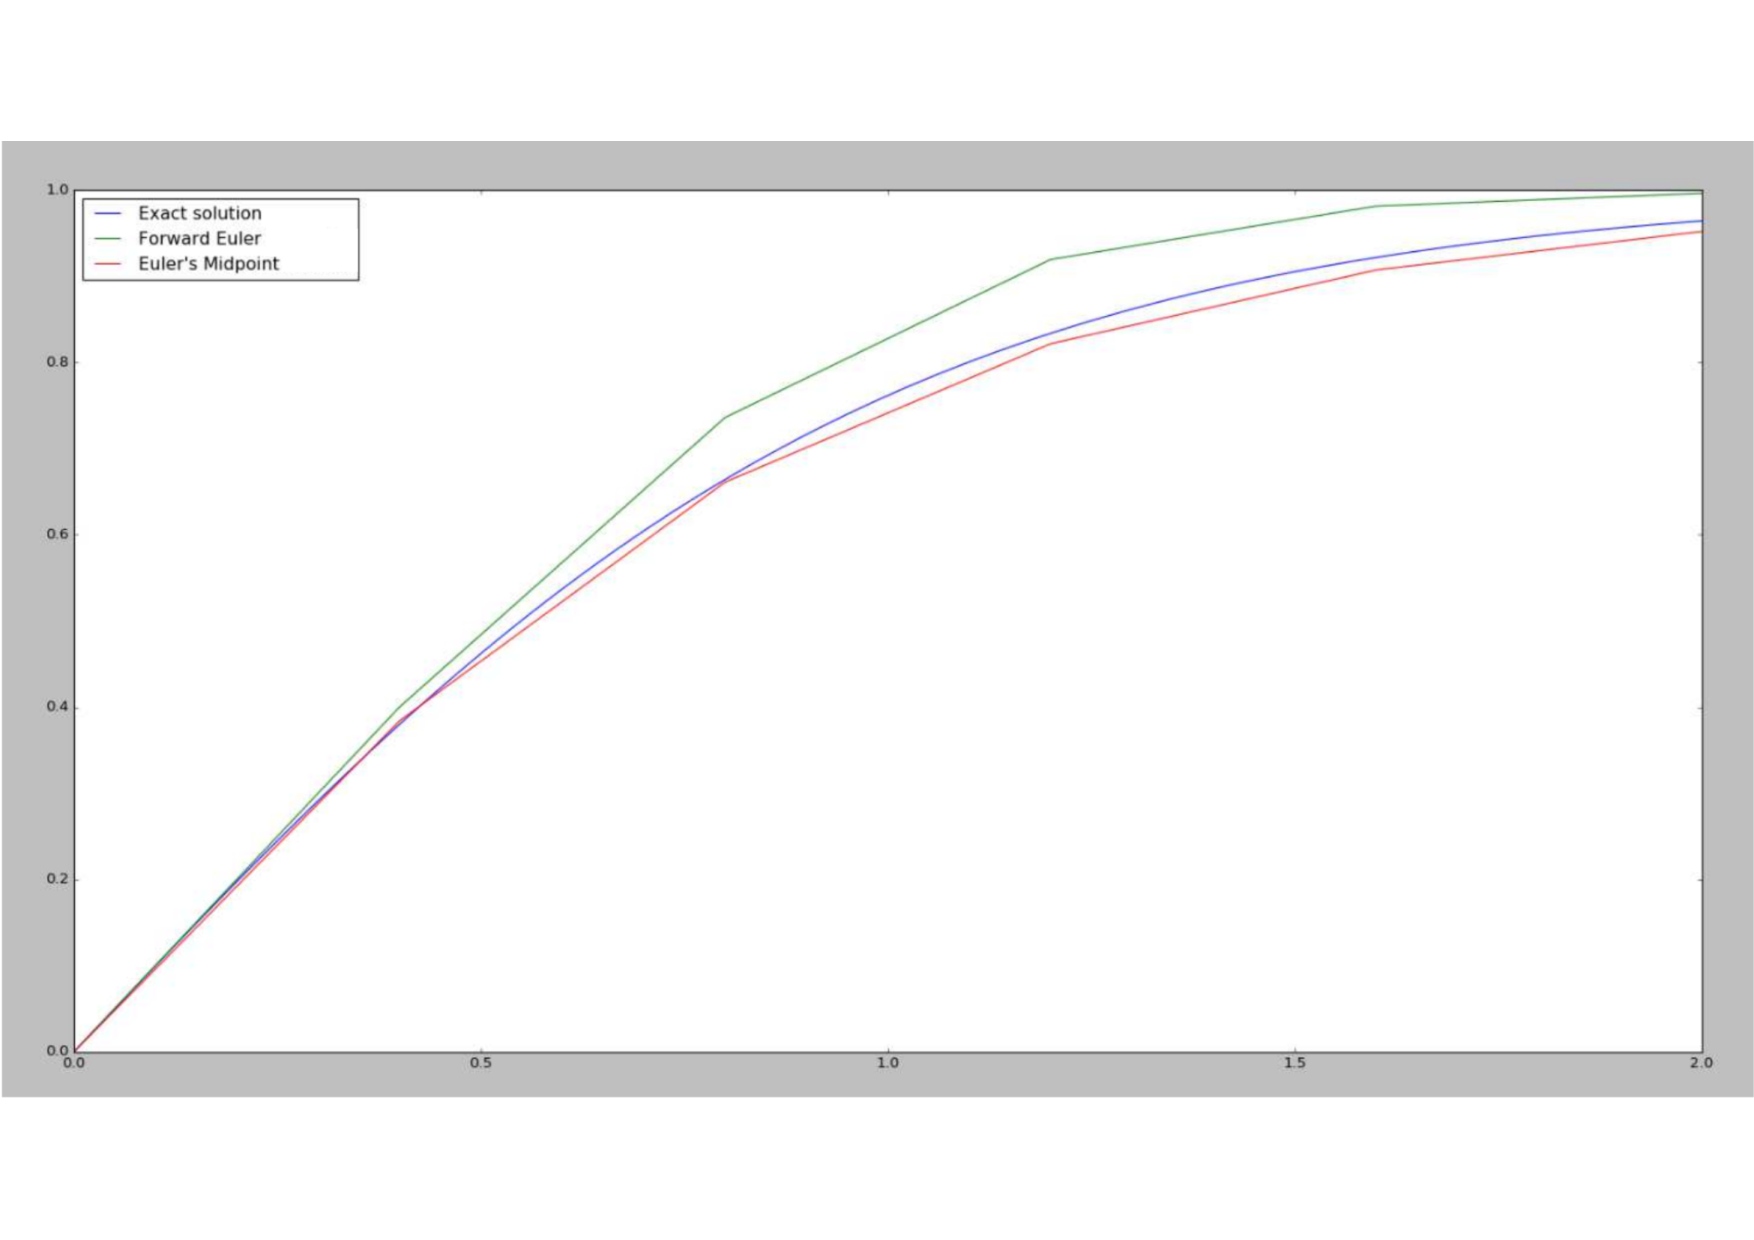
\includegraphics[scale=0.6]{oblig2_2.pdf}

\subsection{)}
Har ligningen:
\[x'(t) + x(t)^{2} = 1\]
og får oppgitt at
\[0 \leq x(t*) < 1\]
Utifra det kan vi se at $x(t*)^{2}$ også må være mindre enn 1.
\[0 \leq x(t*)^{2} < 1\]
Ettersom ligningen adderer $x(t)^{2}$ med $x'(t)$, og svaret skal bli 1, så må $x'(t)$ også være større enn 0, og en positiv verdi for $x'(t)$ vil si at $x(t)$ er voksende. 

x(t) konvergerer mot 1 nedenfra, så $x(t) > 1$ går ikke.
Å sette $x(t) = 1$ vil vel da måtte gi $t = \infty$


\end{document}

